\documentclass[journal,onecolumn]{IEEEtran}

% correct bad hyphenation here
\hyphenation{op-tical net-works semi-conduc-tor}

\usepackage{cite}
\usepackage{amsmath,amssymb,amsfonts}
\usepackage{algorithmic}
\usepackage{graphicx}
\usepackage{textcomp}
\usepackage{xcolor}
\usepackage[brazilian]{babel}
\usepackage[utf8]{inputenc}
\usepackage[T1]{fontenc}
\usepackage{listings}
\usepackage{listings-golang}
\usepackage{color}
\usepackage{float}
\usepackage{multirow}
\usepackage{hyperref}

\definecolor{dkgreen}{rgb}{0,0.6,0}
\definecolor{gray}{rgb}{0.5,0.5,0.5}
\definecolor{mauve}{rgb}{0.58,0,0.82}

\lstset{frame=tb,
  language=Golang,
  aboveskip=3mm,
  belowskip=3mm,
  showstringspaces=false,
  columns=flexible,
  basicstyle={\small\ttfamily},
  numbers=none,
  numberstyle=\tiny\color{gray},
  keywordstyle=\color{blue},
  commentstyle=\color{dkgreen},
  stringstyle=\color{mauve},
  breaklines=true,
  breakatwhitespace=true,
  tabsize=3
}
\lstset{language=Golang}
\def\BibTeX{{\rm B\kern-.05em{\sc i\kern-.025em b}\kern-.08em
    T\kern-.1667em\lower.7ex\hbox{E}\kern-.125emX}}


\begin{document}

\title{Relatório da Atividade 4: Raft}

\author{\IEEEauthorblockN{Isabelle Ferreira de Oliveira}
\IEEEauthorblockA{\textit{CES-27 - Engenharia da Computação 2020} \\
\textit{Instituto Tecnológico de Aeronáutica (ITA)}\\
São José dos Campos, Brasil \\
isabelle.ferreira3000@gmail.com}
}

\maketitle

\begin{abstract}
Esse relatório documenta um trabalho com o protocolo Raft para consenso distribuído. Não será trabalhado com \textit{log replication}.
\end{abstract}

\begin{IEEEkeywords}
Raft, Golang, sistema distribuído
\end{IEEEkeywords}

\section{Implementação}

\subsection{Ao receber um AppendEntry (heartbeat)}
Subsection text here.

\subsubsection{Follower}
\subsubsection{Candidate}
\subsubsection{Leader}

\subsection{Ao receber um RequestVote}
Subsubsection text here.

\subsubsection{Follower}
\subsubsection{Candidate}
\subsubsection{Leader}

\subsection{Ao receber um Reply}
Subsubsection text here.

\subsubsection{Follower}
\subsubsection{Candidate}
\subsubsection{Leader}

\section{Resultados e Conclusões}
The conclusion goes here.

\begin{figure}[H]
\centering
\centerline{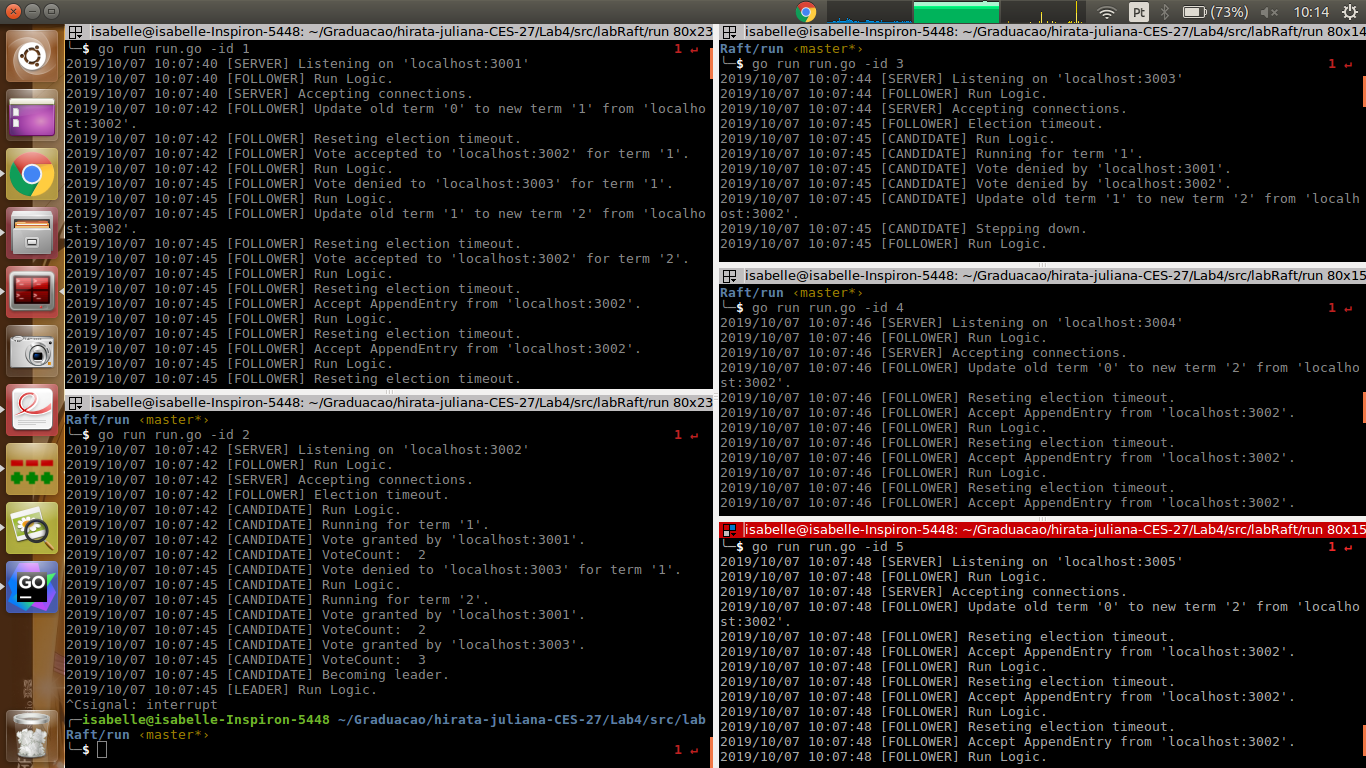
\includegraphics[scale=0.4]{imagens/funcionamento_normal.png}}
\caption{Funcionamento normal para os 5 processos.}
\label{funcionamento_normal}
\end{figure}

\begin{figure}[H]
\centering
\centerline{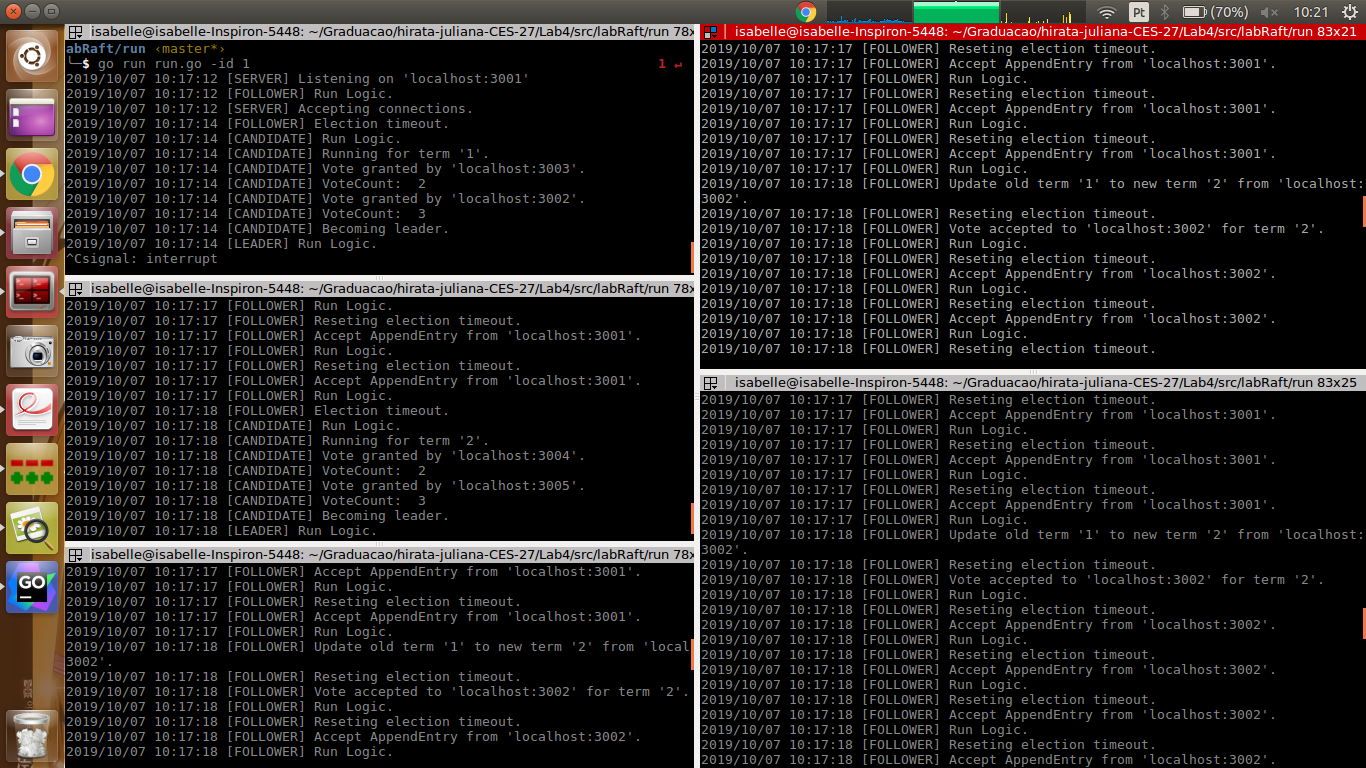
\includegraphics[scale=0.4]{imagens/falha_no_lider.png}}
\caption{Funcionamento após a falha no \textit{leader}, seguido de retomada do processo.}.
\label{falha_no_lider}
\end{figure}

\begin{figure}[H]
\centering
\centerline{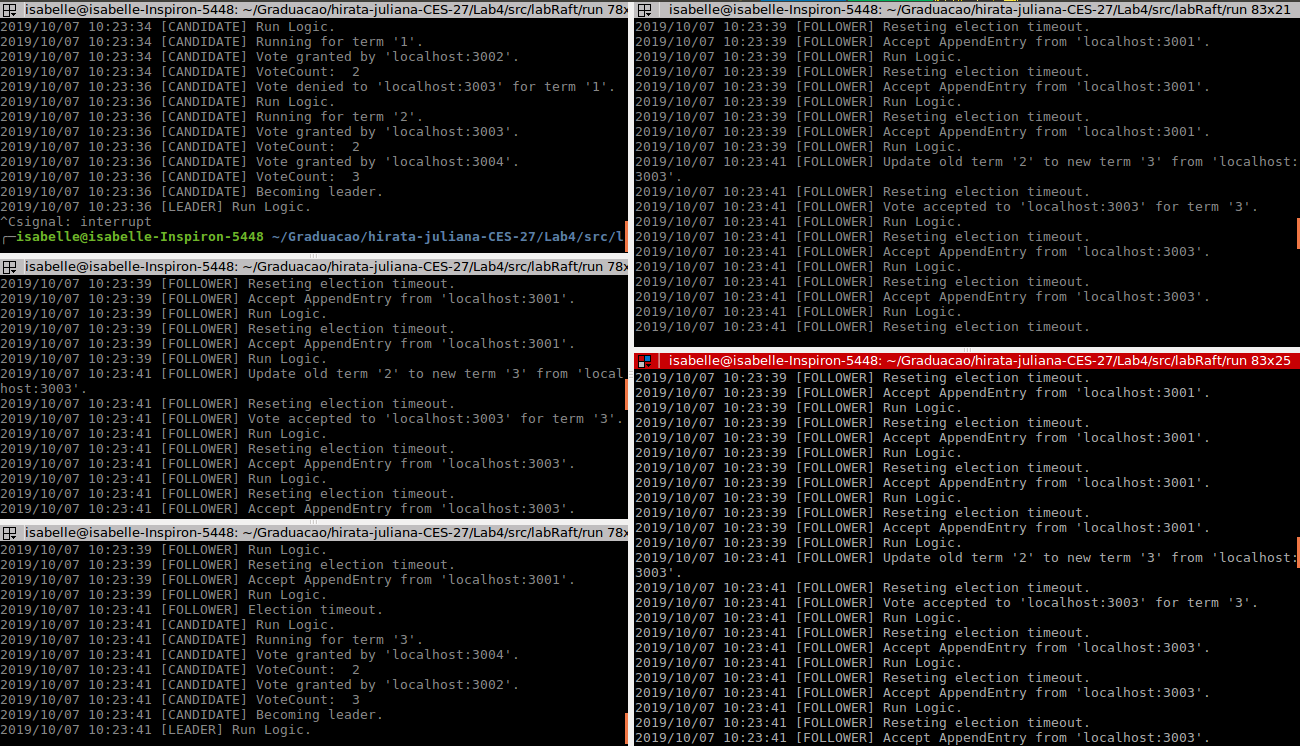
\includegraphics[scale=0.4]{imagens/1_falha.png}}
\caption{Funcionamento após a falha no \textit{leader}.}.
\label{1_falha}
\end{figure}

\begin{figure}[H]
\centering
\centerline{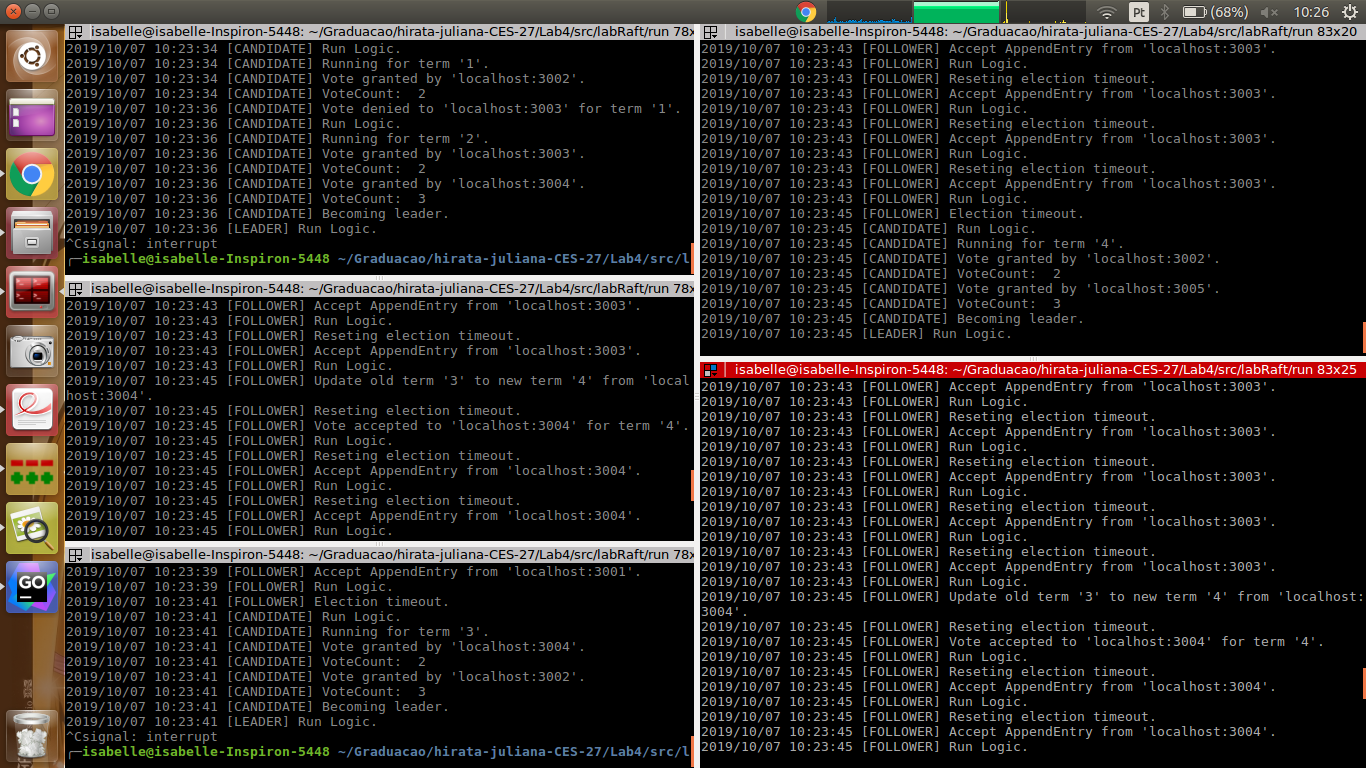
\includegraphics[scale=0.4]{imagens/2_falhas.png}}
\caption{Funcionamento após a falha no próximo \textit{leader}.}.
\label{2_falhas}
\end{figure}

\begin{figure}[H]
\centering
\centerline{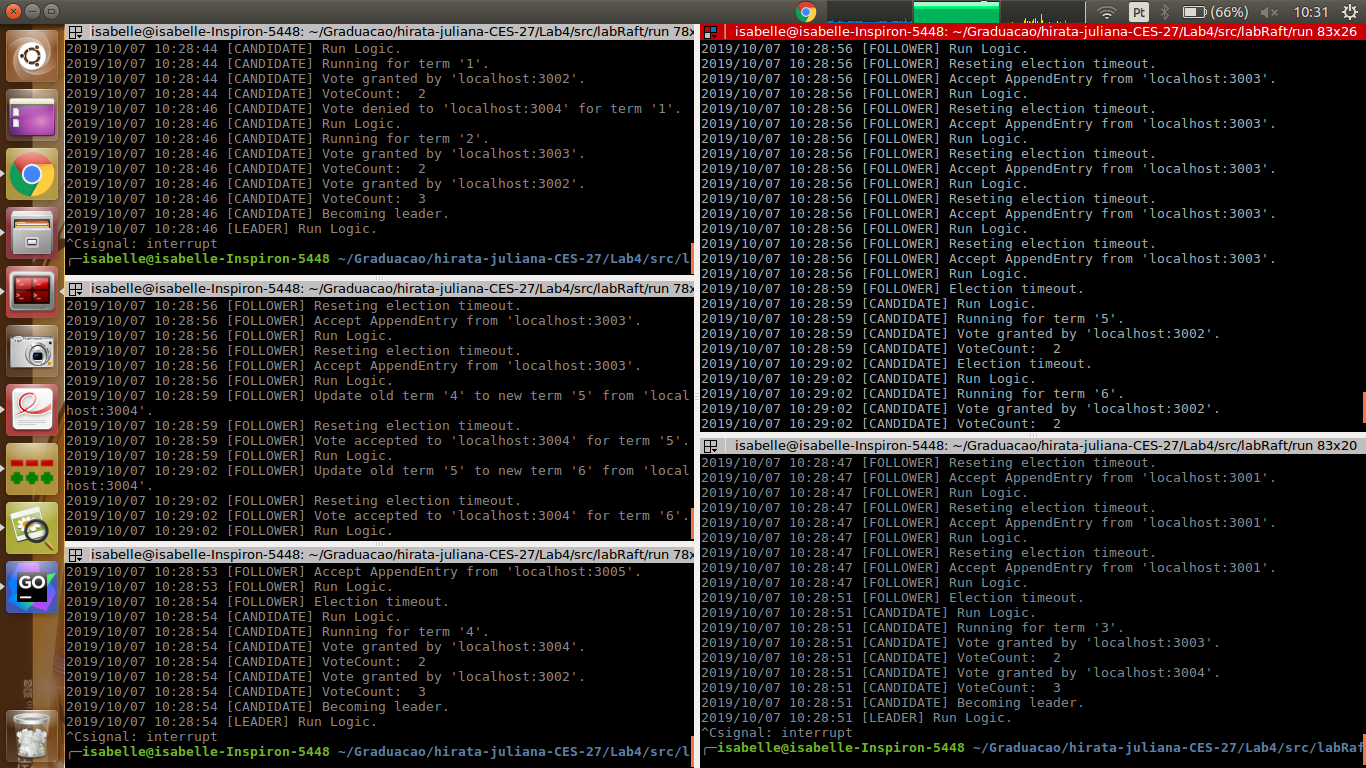
\includegraphics[scale=0.4]{imagens/3_falhas.png}}
\caption{Funcionamento após a falha no terceiro \textit{leader}. Note que o sistema não consegue mais decidir por um novo \textit{leader}.}.
\label{3_falhas}
\end{figure}

\end{document}
